\documentclass[tikz,border=2pt]{standalone}
\usepackage{amsmath,amssymb}
\usepackage{tikz}

\begin{document}
% The power set of {a, b, c}: all 2^3 = 8 subsets, drawn by inclusion.
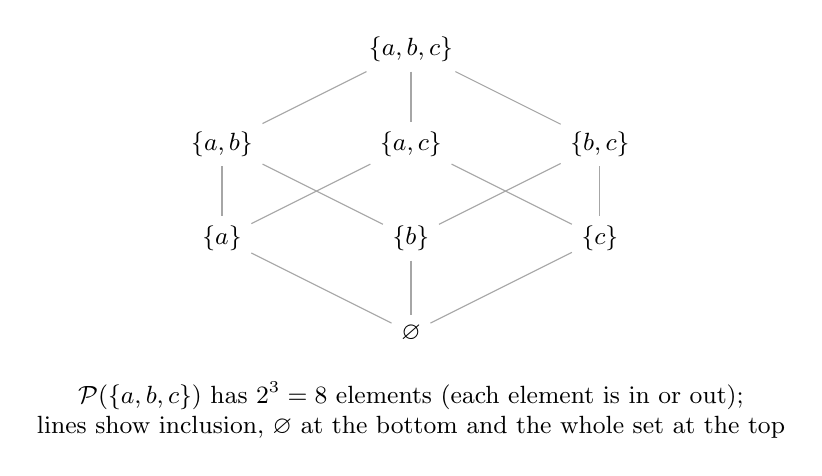
\begin{tikzpicture}[every node/.style={font=\small}]
	\node (top) at (0,3.6) {$\{a,b,c\}$};
	\node (ab) at (-2.4,2.4) {$\{a,b\}$};
	\node (ac) at (0,2.4) {$\{a,c\}$};
	\node (bc) at (2.4,2.4) {$\{b,c\}$};
	\node (a) at (-2.4,1.2) {$\{a\}$};
	\node (b) at (0,1.2) {$\{b\}$};
	\node (c) at (2.4,1.2) {$\{c\}$};
	\node (e) at (0,0) {$\varnothing$};
	\foreach \u/\v in {top/ab, top/ac, top/bc, ab/a, ab/b, ac/a, ac/c, bc/b, bc/c, a/e, b/e, c/e} {\draw[gray!70] (\u) -- (\v);}
	\node[anchor=north, align=center] at (0,-0.5) {$\mathcal{P}(\{a,b,c\})$ has $2^3=8$ elements (each element is in or out);\\ lines show inclusion, $\varnothing$ at the bottom and the whole set at the top};
\end{tikzpicture}
\end{document}
